\chapter{Revealing Object Interactions with \textsc{PathObjects}}
\chaptermark{Revealing Object Interactions}
\label{c:approach}

\section{Concept}

\section{Diagram Notation}
\subsection{Basic Concept}
\subsection{Diagram Aesthetics}
The object communication diagrams of \textsc{PathObjects} form graph structures, whereby  objects constitute nodes, and the arrows representing messages constitute edges.
Graph drawing is a research area with a long history of its own, and there is broad consent about the aesthetic properties that should be aimed at in order to maximize perceivability \cite{battista_graph_1998, kaufmann_drawing_2001, diehl_software_2007}.
Consequently, it stands to reason that these criteria should also be applied to our interactive object communication diagrams.
The seven most important criteria are presented in the following.

\paragraph{Crossing Minimization} User studies suggest that the most important aesthetic criterion is the minimization of edge crossings \cite{purchase_effective_2000, purchase_graph_2004, purchase_graph_2010}.
The more edges cross each other, the harder it becomes for the human eye to keep track of which nodes are connected by an edge.
Graph drawings that do not entail edge crossings are called planar, and are regarded as the best-case scenario.
But although planar graph drawing algorithms are comparatively simple, the excessive optimization of drawings in these premises will most likely interfere with other aesthetic criteria.

\paragraph{Bend Minimization} Bends make it harder for the human eye to follow the route of an edge.
Consequently, both the maximum number of bends on a single edge as well as the total number of bends on all edges should be as low as possible.
Furthermore, the variance of the number of bends on edges should be minimized.
However, recent studies suggest that continuity is more important than the number of bends \cite{diehl_software_2007}.

\paragraph{Length Minimization} Similar to crossings and bends, increasing edge lengths make it increasingly difficult for the viewer of a graph drawing to follow their paths.
Therefore, both the length of the longest edge and the total edge length should be minimized.
In addition, some authors state that the overall variance of lengths should be minimized in order to provide uniform edge lengths.

\paragraph{Area Minimization} The minimization of the area a diagram takes up is especially important when it cannot be scaled down arbitrarily.
This is the case with \textsc{PathObjects} diagrams, since textual information associated with nodes and edges has to stay above perceptive thresholds and may not overlap.
Furthermore, the efficient utilization of screen space is important.
Although our interactive information presentation offers scrolling functionality and thus allows diagram extents to exceed the viewport, scrolling interferes with reading the diagram and consequently complicates the assimilation of information.

\paragraph{Symmetry} Nodes should be distributed evenly on the canvas and thus should form a homogeneous density.
Furthermore, if the underlying graph structure features symmetries, these symmetries should also be reflected by the graph drawing.

\paragraph{Clustering} Interconnected parts of a graph should be drawn distinguishable from other so-called clusters.
In our case, connections are established through message exchanges, and objects or respectively nodes are connected stronger if they exchange more messages among each other than with other objects.
In addition, the edges between members of the same cluster should be shorter than edges that connect nodes from different clusters.

\paragraph{Orthogonality} Some authors state that fixing nodes and edges to an orthogonal grid improves the understandability of graph drawings \cite{sugiyama_methods_1981, batini_what_1985}.
And although Purchase et al. could not find significant evidence for this claim in a user study \cite{purchase_which_1997}, the majority of participants that were confronted with different variations of UML collaboration diagrams in another study nevertheless favored this edge routing strategy over other approaches \cite{purchase_graph_2004}.

Most of those drawing optimization criteria are NP-hard computational problems for tree structures \cite{battista_graph_1998}.
And since the graphs that should be presented through our interactive communication diagrams are call trees, this raises the question if the immediate character of the underlying tracing approach can be maintained.
For that reason, a runtime performance evaluation of the diagram construction is presented in Section \ref{s:DiscussionPerformance}.

So far, the presented aesthetic criteria are generally valid for all graph drawings regardless of their specific purpose.
In addition, Purchase et al. analyzed the user preferences and perceivability impacts of different variations of UML communication diagrams \cite{purchase_uml_2002, purchase_graph_2004}.
Since our interactive diagram notation is very similar to communication diagrams, the results of those studies also were taken into account.
\todo{blubb}

\subsection{Automatic Diagram Layout}
In general, there are many profound arguments for generating diagram layouts automatically.
For instance, automated drawing of diagrams has the side-effect that conformance to a certain style guide .
Furthermore, the costs of communication and thus the total costs of production and maintenance can be reduced by use of automated drawing of diagrams.
But the strongest reason to rely on the automated generation of diagram layouts becomes evident when taking the intended use of \textsc{PathTools} into account.


\section{Interactive Components}

\subsection{Navigation}
\subsubsection{Temporal Navigation}
\begin{figure}[tb]
	\centering
	
	\begin{subfigure}[b]{0.45\textwidth}
		\centering
        
\includegraphics[width=\textwidth]{../images/04-ImplTimeline1}
        \caption[Default View]{}
		\label{fig:ImplementationTimelineDefault}
	\end{subfigure}
	\quad
	\begin{subfigure}[b]{0.45\textwidth}
		\centering
		
\includegraphics[width=\textwidth]{../images/04-ImplTimeline2}
		\caption[Search Result Highlighting]{}
		\label{fig:ImplementationTimelineSearch}
	\end{subfigure}
	\quad
	\begin{subfigure}[b]{0.45\textwidth}
		\centering
		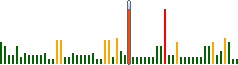
\includegraphics[width=\textwidth]{../images/04-ImplTimeline3}
		\caption[Differing Metrics Applied to Item Height and Color]{}
		\label{fig:ImplementationTimelineMetrics}
	\end{subfigure}
	
	\caption[Variations of the Timeline View]{Three variations of the timeline view that show the exact same execution history; in each case, the current step is highlighted and the according return point is marked in red.
		a) Default view with mapping of stack depth to item height.
		b) Search result highlighting.
		c) Differing metrics applied to item height and item color.
	}
	\label{fig:ImplementationTimeline}
\end{figure}

Figure \ref{fig:ImplementationTimeline} shows examples of the timeline view.
Each bar represents a step of the execution history, or respectively either a message send or the return from a message send.
The alignment along the horizontal axis corresponds to the chronological order of appearances.
The current step is marked with a blue overlay, and the corresponding send or return step is marked in red.
Developers can use the timeline to navigate through the execution history by either selection a specific step, by using the keyboard's left and right arrows, or by clicking the arrows that are displayed alongside the timeline.

All three examples in Figure \ref{fig:ImplementationTimeline} show the exact same execution history at the exact same point of the execution.
Figure \ref{fig:ImplementationTimelineDefault} represents the default configuration of the timeline view.
In this case, the height of the single timeline items corresponds to the depth of the call stack.
However, the concept of information layers (cf. \ref{??}\todo{cite}) allows to map arbitrary metrics to this dimension of the diagram.
Figure \ref{fig:ImplementationTimelineSearch} shows how search results are highlighted within the timeline.
In the depicted example, the developer performed a search for occurrences of the \inlinecode{attach:} message.
Two matches are found, whereby each consists of a send and a returns step.
These occurrences correspond to the registration of the analog and digital clock instances at the clock timer.
Figure \ref{fig:ImplementationTimelineMetrics} illustrates the usage of information layers in conjunction with the timeline view.
The height of the items now no longer represents the stack depth, but the number of variable accesses in each method.
The color of the items indicates the lines of code of each message.
One can see that the current step is the one with by far the most variable accesses.
Furthermore, the visualization indicates that most methods have an acceptable length, with the exception of the method that is the implementation of the selected message.

\subsubsection{Spatial Navigation}
\subsubsection{}

\subsection{Exploration}
\subsection{Focusing}

\subsection{Information Layers}
Program comprehension usually does not end in itself but rather serves a specific purpose.
Consequently, the situations in which developers try to build an understanding of a software system are manifold.
Furthermore, different purposes require different additional information that can assist developers in specific situations.

For instance, if a developer wants to fix a defect, information such as recent changes that have been made to the system might be of interest.
Furthermore, one might want to display root cause probabilities along with methods.
In contrast, if the goal is a general refactoring to improve the overall code quality, one might be interested in metrics like lines of code or cyclomatic complexity.
The elimination of performance bottlenecks constitutes another common scenario.
In this case, developers most likely are interest in runtime profiling data.